\documentclass{article}
\usepackage[normalem]{ulem}
\usepackage[12pt]{extsizes}
\usepackage[utf8]{inputenc}
\usepackage[T2A]{fontenc}
\usepackage{amsmath}
\usepackage{amssymb}
\usepackage{hyperref}
\usepackage{amsfonts}
\usepackage{cmap}
\usepackage{multicol}
\usepackage{comment}
\usepackage{listings}
\usepackage{color}
\usepackage{colortbl}
\definecolor{bkgreen}{rgb}{0.0, 0.26, 0.15}
\usepackage[parfill]{parskip}

\usepackage{xcolor}
\usepackage[left=1.5cm,right=2cm,top=2cm,bottom=2cm,bindingoffset=0.1cm]{geometry}
\usepackage[russian]{babel}
\usepackage[pdf]{graphviz}
\usepackage{tikz}
\usepackage{etoolbox} % <--- added


\DeclareRobustCommand{\divby}{%
\mathrel{\text{\vbox{\baselineskip.65ex\lineskiplimit0pt\hbox{.}\hbox{.}\hbox{.}}}}%
}
\AtBeginEnvironment{enumerate}{\linespread{.84}\selectfont}
\newcommand{\ctd}{\begin{flushright} $\square$ \end{flushright}}

\usepackage{amsthm}
\usepackage{mathtools}
\usepackage{textcomp}
\usepackage{tikz}

%\theoremstyle{definition} % жирный заголовок, плоский текст
\newtheorem{Thm}{\underline{Теорема}} % нумерация будет "<номер subsection>.<номер теоремы>"
\newtheorem{Lm}[Thm]{\underline{Лемма}} % Нумерация такая же, как и у теорем
\newtheorem{Ex}[Thm]{Упражнение} % Нумерация такая же, как и у теорем
\newtheorem{Task}[Thm]{Задача} % Нумерация такая же, как и у теорем
\newtheorem{Example}{Пример}[section] % Нумерация такая же, как и у теорем
\newtheorem{Code}[Thm]{Код} % Нумерация такая же, как и у теорем
%\theoremstyle{plain} % жирный заголовок, курсивный текст
\newtheorem{Def}{Определение} % Нумерация такая же, как и у теорем

\newtheorem{Cons}[Thm]{Следствие} % Нумерация такая же, как и у теорем
\newtheorem{Conj}[Thm]{Гипотеза} % Нумерация такая же, как и у теорем
\newtheorem{Prop}[Thm]{Утверждение} % Нумерация такая же, как и у теорем
\newtheorem{Rem}{Замечание} % Нумерация такая же, как и у теорем
\newtheorem{Remark}[Thm]{Замечание} % Нумерация такая же, как и у теорем
\newtheorem{Img}[Thm]{Иллюстрация} % Нумерация такая же, как и у теорем

\newcommand{\deff}[1]{\underline{\textbf{#1}}}
\newcommand{\thmm}[1]{\underline{\textbf{#1}}}
\newcommand*\xor{\mathbin{\oplus}}
\newcommand{\mytilde}{\raisebox{0.5ex}{\texttildelow}}

\makeatletter
\renewcommand*\env@matrix[1][*\c@MaxMatrixCols c]{%
  \hskip -\arraycolsep
  \let\@ifnextchar\new@ifnextchar
  \array{#1}}
\makeatother

\hypersetup{
    colorlinks=true,
    linkcolor=black,
    filecolor=magenta,      
    urlcolor=blue,
    pdftitle={Linear Algebra semestr 2},
    pdfpagemode=FullScreen,
    }

\lstset{ %
  language=C++, % the language of the code
  basicstyle=\footnotesize\ttfamily, % the size of the fonts that are used for the code
  numbers=left, % where to put the line-numbers
  numberstyle=\footnotesize\color{black},  % the style that is used for the line-numbers
  stepnumber=0, % the step between two line-numbers. If it's 1, each line 
       % will be numbered
  numbersep=0.7em,       % how far the line-numbers are from the code
  backgroundcolor=\color{white!95!gray}, % choose the background color. You must add \usepackage{color}
  showspaces=false,      % show spaces adding particular underscores
  showstringspaces=false,% underline spaces within strings
  showtabs=false,        % show tabs within strings adding particular underscores
  frame=single, % adds a frame around the code
  rulecolor=\color{black},        % if not set, the frame-color may be changed on line-breaks within not-black text (e.g. commens (green here))
  tabsize=2,    % sets default tabsize to 2 spaces
  %captionpos=b,% sets the caption-position to bottom
  breaklines=true,       % sets automatic line breaking
  breakatwhitespace=false,        % sets if automatic breaks should only happen at whitespace
  %title=\lstname,       % show the filename of files included with \lstinputlisting;
       % also try caption instead of title
  identifierstyle=\color{black!50!green},  
  keywordstyle=\color{blue},      % keyword style
  commentstyle=\color{gray},      % comment style
  stringstyle=\color{purple},      % string literal style
  escapeinside={\%*}{*)},% if you want to add a comment within your code
  morekeywords={n,k},    % if you want to add more keywords to the set
  morecomment=[l][\color{black!50!green}]{\#}, % to color #include<cstdio> 
  morecomment=[s][\color{gray!50!black}]{/**}{*/}
}


% Разные определения
\newcommand{\abs}[1]{\left|{#1}\right|}
\newcommand{\norm}[1]{\lVert{#1}\rVert}
\newcommand{\stk}[2]{\stackrel{\eqref{#1}}{#2}}
\newcommand{\D}{\Delta}
\newcommand{\pderiv}[2]{\frac{\partial #1}{\partial #2}}
\newcommand{\appr}[1]{\xrightarrow[#1]{}}
\newcommand{\scal}[1]{\left\langle #1 \right\rangle}
\newcommand{\F}{\mathcal{F}}


% Числовые множества
\newcommand{\R}{\mathbb{R}}
\renewcommand{\C}{\mathbb{C}}
\newcommand{\N}{\mathbb{N}}
\newcommand{\Q}{\mathbb{Q}}
\newcommand{\Z}{\mathbb{Z}}


% Необходимость, достаточность
\newcommand{\nec}{{$\Rightarrow$}}
\newcommand{\suff}{{$\Leftarrow$}}


% Буквенные \Re и \Im
\DeclareMathOperator{\@custom@Re}{Re}
\DeclareMathOperator{\@custom@Im}{Im}
\renewcommand{\Re}{\@custom@Re}
\renewcommand{\Im}{\@custom@Im}

% Еще переопределения
\renewcommand{\emptyset}{\varnothing}

% Математические операторы
\DeclareMathOperator{\rank}{rank}
\DeclareMathOperator{\mes}{mes}
\DeclareMathOperator{\diam}{diam}
\DeclareMathOperator{\fix}{fix}
\DeclareMathOperator{\sgn}{sgn}
\DeclareMathOperator{\sign}{sgn}
\DeclareMathOperator{\vp}{v.p.}
\DeclareMathOperator{\Arg}{Arg}
\DeclareMathOperator{\Ln}{Ln}
\DeclareMathOperator{\Arcsin}{Arcsin}
\DeclareMathOperator{\Arccos}{Arccos}
\DeclareMathOperator{\Arctg}{Arctg}
\DeclareMathOperator{\Arcctg}{Arcctg}
\DeclareMathOperator{\Arsh}{Arsh}
\DeclareMathOperator{\Arch}{Arch}
\DeclareMathOperator{\Arth}{Arth}
\DeclareMathOperator{\Arcth}{Arcth}

\usepackage{dsfont}
\newcommand{\zero}{\mathds{O}}
\renewcommand{\ker}{\mathcal{K}er}
\newcommand{\rg}{rg}
\renewcommand{\span}{span}

% Интегралы до бесконечности
\newcommand{\iinf}[1]{\int\limits_{#1}^{+\infty}}
\newcommand{\ioinf}{\int\limits_{0}^{+\infty}}
\newcommand{\ipminf}{\int\limits_{-\infty}^{+\infty}}

\newcommand{\Sim}{\text{Sim }}
\newcommand{\Alt}{\text{Alt }}

\newenvironment{Word}[2]{
    \vspace{2pt}
    \textbf{words:}
    \vspace{-7pt}
    \begin{multicols}{#1}
    \begin{enumerate}[#2]       
}{\end{enumerate}\end{multicols}}

\usepackage{lipsum} % sample text
\usepackage{wrapfig}
\usepackage{minted}
\setminted{
    linenos=true,
    frame=leftline,
    fontsize=\ttfamily\small,
    framesep=4mm,
    numbersep=4pt,
    tabsize=4,
    breaklines=true,
    breakautoindent=true
}

\usepackage{subfiles}
\usepackage{fancyhdr}
\pagestyle{fancy}
\fancyhf{}

\fancyhead[C]{Линейная Алгебра} % Центральный заголовок
\fancyhead[L]{КТ ИТМО - 2 Семестр}
\fancyhead[R]{Кучерук Екатерина}


\title{Разбор КР по Линейным отображениям.}
\author{Чепелин Вячеслав}
\date{}

\begin{document}
\maketitle
\tableofcontents
\newpage

\section{Задание 1.}

Это задание в целом на понимание того, как работают функции.

\deff{1.} В пространстве трехмерных геометрических векторов $\mathcal{A}\overline{x} = \overline{x}\times \overline{a}$, где $a = (1,-1, 2)^T$. Найти матрицу оператора $\mathcal{A}$ в базисе $b$, найти $\ker A$ и $\Im A$. $b_1 = (1,1,1)^T, b_2= (1,2,3)^T, b_3 = (1,3,6)^T$.

\textbf{Решение:}

Мы можем плясать от определения матрицы оператора. Для этого нам надо посчитать $\mathcal{A}b_i$, но нам надо не забыть перевести отображение в базис $b$(так как обычно мы считаем в базисе пространства).

$\mathcal{A}b_1 = \begin{pmatrix}
    3 \\
    -1 \\
    -2
\end{pmatrix}$,
$\mathcal{A}b_2 = \begin{pmatrix}
    7 \\
    1 \\
    -3
\end{pmatrix}$, $\mathcal{A}b_3 = \begin{pmatrix}
    12\\
    4\\
    -4
\end{pmatrix}$

Замечу, что это произведение в обычном базисе $V_3$. Поэтому каждый вектор мы должны еще перевести его в $x'$. Это можно например сделать с помощью обратной матрицы $x' = T^{-1}x$. Посчитаем обратную, она нам понадобится еще во втором (более простом) решении. 
$$T^{-1} = (T)^{-1} = \begin{pmatrix}
    1 & 1 & 1 \\
    1 & 2 & 3 \\
    1 & 3 & 6
\end{pmatrix}^{-1} = \begin{pmatrix}
    3 & -3 & 1 \\
    -3& 5 &-2 \\
    1 & -2 & 1 \\
\end{pmatrix}$$

Тогда $b_1' =\begin{pmatrix}
    10 \\
    -10 \\
    3
\end{pmatrix}, b_2' = \begin{pmatrix}
    15 \\
    -10\\
    2
\end{pmatrix}, b_3' =\begin{pmatrix}
    20 \\
    -8\\
    0
\end{pmatrix}$

Ранг этой системы векторов $2$, так что мы нигде не ошиблись. Поставим эти векторочки столбиками в матрицу и получим матрицу 

Второ решение состоит в том, что мы могли пойти по-другому пути и посчитать матрицу в исходном базисе $e_1,e_2,e_3$, а потом воспользоваться формулой замены базиса $A' =T^{-1}AT$.

Подставим $e_1,e_2,e_3$ получим:
$$\mathcal{A}e_1 = \begin{pmatrix}
    0\\
    -2\\
    -1
\end{pmatrix}, \mathcal{A}e_2 = \begin{pmatrix}
    2 \\
    0 \\
    -1 \\
\end{pmatrix}, \mathcal{A}e_3 =  \begin{pmatrix}
    1 \\
    1 \\
    0
\end{pmatrix}$$
Зная $T$ и $T^{-1}$ получаем тот же ответ.

Так вот, теперь давайте найдем $\ker$ и $\Im$. Можно воспользоваться только что найденными векторами и выбрать 2 из них. Так же, чтобы найти $\ker$ мы можем просто взять наш вектор $a$.

\newpage
\section{Задание 2.}

\deff{1.} Доказать, что матрица $\mathcal{A}$ - матрица о.п.с. Найти спектральное разложение $\mathcal{A}$ и вычислить с его помощью $\exp A$.

$\mathcal{A} = \begin{pmatrix}
    -4 & -3 & 0 \\
    12 & 7 & 2 \\
    0 & 2 & -2 \\
\end{pmatrix}, \lambda_1 = -1, \lambda_2 = 0$ - собственные числа $A$.

\textbf{Решение:}

Для начала найдем еще одно собственное число(или кратность). Для этого вспомним формулу $tr \mathcal{A}$ или $\det A $ через собственные числа.
$$tr \mathcal{A} = tr A = -4 + 7 + -2 = 1 = \lambda_1 + \lambda_2 + \lambda_3 = -1 + 0 + \lambda_3 \Leftrightarrow 1 = -1 + \lambda_3 \Leftrightarrow \lambda_3 = 2$$
Откуда мы нашли третью $\lambda$. Если вдруг вы забыли это, то считаете характеристический. В данном случае $\chi(t) = 
-t^3+t^2+2t = -t(t-2)(t+1)$

Вспомним теорему, что $1\leq\gamma(\lambda)\leq\alpha(\lambda)$. То есть $\gamma(\lambda_i) = 1$ для данных $\lambda$, откуда $\sum\limits_{\lambda}\gamma(\lambda) = n = 3 = \dim V$, то есть в данном случае это о.п.с.

Теперь посчитаем спектральное разложение. Буду считать его не в тупую, а через разложение единицы.
$$\cfrac{1}{x(x+1)(x-2)} = \cfrac{\alpha_1}{x} + \cfrac{\alpha_2}{(x+1)} + \cfrac{\alpha_3}{(x-2)}$$
Считая разложение на простые дроби получаем:
$\alpha_1 = -\cfrac{1}{2}, \alpha_2 = \cfrac{1}{3}, \alpha_3 = \cfrac{1}{6}$. 

Интересный факт. $\mathcal{A}$ уже сам считается проектором на $V_{0}$, так что его считать нам не надо.

$P_{1} = \cfrac{1}{3} (\mathcal{A}- 2\varepsilon)(\mathcal{A})$

$P_2 = E-P_1-P_0 $

Зная это уже легко досчитывается сами проекторы. $A = \sum\limits_{\lambda}\lambda P_\lambda$.

А функция считается еще проще $A = \sum\limits_{\lambda} e^\lambda P_\lambda$

\newpage

\section{Задание 3.}

\deff{1.} Найти $\chi, \varphi,\lambda,\alpha,\gamma, m, V_{\lambda}, K_{\lambda}$. Подобна ли матрица диагональной, если нет выписать Жорданову форму.

$A = \begin{pmatrix}
    4 & 6 & -15 \\
    1& 3  & -5 \\
    1 & 2 & -4 \\
\end{pmatrix}$

\textbf{Решение:}

Давайте найдем собственные числа. Как мы знаем из теоремы Виета:
$$\begin{cases}
    \lambda_1 + \lambda_2 + \lambda_3 = tr A = 3\\
    \lambda_1 \cdot \lambda_2 \cdot \lambda_3 = \det A = 1
\end{cases}$$
Если заметить, то у нас одно собственное число $ = 1$. Откуда сразу получаем характеристический $\chi(t) = -(t-1)^3$. Теперь давайте найдем $m(1)$. Заметим, что он не равен одному. Максимум он может быть равен трем. Посмотрим на $(\mathcal{A}-\varepsilon)^2$. Ой это ноль, откуда $m(1) = 2$. Откуда из вычислений получаем, что $\gamma(2)= 2$. Матрица у нас сразу не диагональная.

$V_\lambda$ найдем как обычно $K_\lambda$ в данном случае равен $V$. $\varphi = (t-1)^{m(1)}=(t-1)^2$. Отсюда уже можно понять Жорданову форму.

\newpage
\section{Задание 4.}

Оно настолько очевидное из теории, что я не знаю, что сюда писать













\newpage
\section{Информация о курсе}

Поток — y2024.\newline
Группы M3138-M3139.\newline
Преподаватель --- Кучерук Екатерина Аркадьевна.\par

Данный разбор сделан не в коммерческих целях, я не хочу никого обидеть, я просто пишу конспекты для себя плак плак плак
\begin{center}
   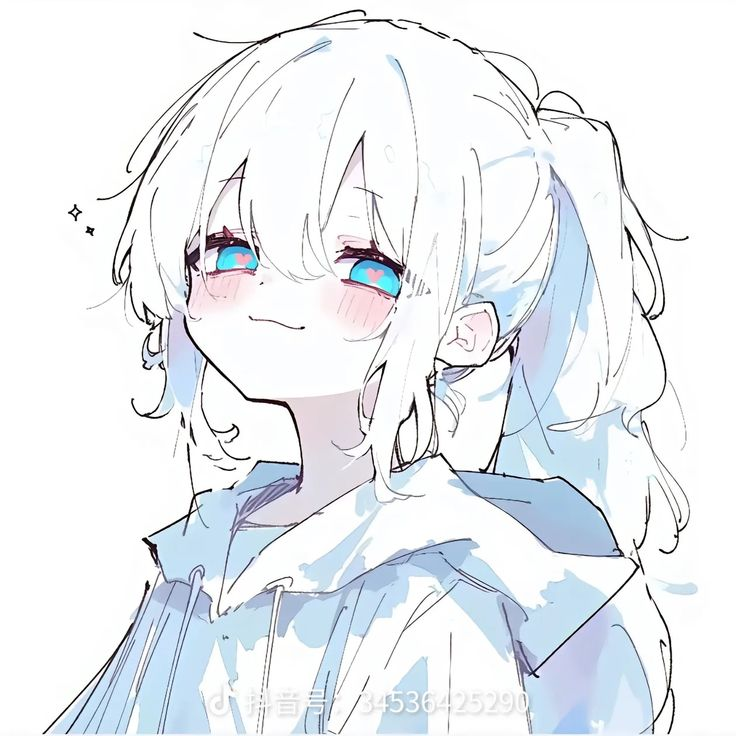
\includegraphics[height=17cm]{assets/cute-girl.jpg}
\end{center}

\end{document}
